\let\negmedspace\undefined
\let\negthickspace\undefined
\documentclass[journal]{IEEEtran}
\usepackage[a5paper, margin=10mm, onecolumn]{geometry}
%\usepackage{lmodern} % Ensure lmodern is loaded for pdflatex
\usepackage{tfrupee} % Include tfrupee package

\setlength{\headheight}{1cm} % Set the height of the header box
\setlength{\headsep}{0mm}     % Set the distance between the header box and the top of the text

\usepackage{gvv-book}
\usepackage{gvv}
\usepackage{cite}
\usepackage{amsmath,amssymb,amsfonts,amsthm}
\usepackage{algorithmic}
\usepackage{graphicx}
\usepackage{textcomp}
\usepackage{xcolor}
\usepackage{txfonts}
\usepackage{listings}
\usepackage{enumitem}
\usepackage{mathtools}
\usepackage{gensymb}
\usepackage{comment}
\usepackage[breaklinks=true]{hyperref}
\usepackage{tkz-euclide} 
\usepackage{listings}
% \usepackage{gvv}                                        
\def\inputGnumericTable{}                                 
\usepackage[latin1]{inputenc}                                
\usepackage{color}                                            
\usepackage{array}                                            
\usepackage{longtable}                                       
\usepackage{calc}                                             
\usepackage{multirow}                                         
\usepackage{hhline}                                           
\usepackage{ifthen}                                           
\usepackage{lscape}
\usepackage{multicol}
\begin{document}

\bibliographystyle{IEEEtran}
\vspace{3cm}

\title{12.26}
\author{EE25BTECH11012-BEERAM MADHURI}
% \maketitle
% \newpage
% \bigskip
{\let\newpage\relax\maketitle}

\renewcommand{\thefigure}{\theenumi}
\renewcommand{\thetable}{\theenumi}
\setlength{\intextsep}{10pt} % Space between text and floats


\numberwithin{equation}{enumi}
\numberwithin{figure}{enumi}
\renewcommand{\thetable}{\theenumi}


\textbf{Question}:\\
Phani starts from point $\mathbf{P}$, goes North for $3$ km, and then East for $4$ km to reach point $\mathbf{Q}$. She then turns to face point $\mathbf{P}$ and goes $15$ km in that direction. She then goes North for $6$ km. How far is she from point $\mathbf{P}$, and in which direction should she go to reach point $\mathbf{P}$?

\begin{enumerate}
    \item[a)] $8$ km, East
    \item[b)] $12$ km, North
    \item[c)] $6$ km, East
    \item[d)] $10$ km, North
\end{enumerate}
\textbf{Solution:}\\
Let point $\mathbf{P}$  be the origin:
\begin{align}
\mathbf{P} = \begin{bmatrix} 0 \\ 0 \end{bmatrix}
\end{align}
Moving from  $\mathbf{P}$ to $\mathbf{Q}$\\
First, move North by 3 km:
\begin{align}
\mathbf{A} = \begin{bmatrix} 0 \\ 3 \end{bmatrix}
\end{align}

Then, move East by 4 km:
\begin{align}
\mathbf{B} = \begin{bmatrix} 4 \\ 0 \end{bmatrix}
\end{align}

Position at point  $\mathbf{Q}$ is:
\begin{align}
\mathbf{Q} = \mathbf{P} + \mathbf{A} + \mathbf{B} \\= \begin{bmatrix} 0 \\ 0 \end{bmatrix} + \begin{bmatrix} 0 \\ 3 \end{bmatrix} + \begin{bmatrix} 4 \\ 0 \end{bmatrix} \\= \begin{bmatrix} 4 \\ 3 \end{bmatrix}
\end{align}

Move 15 km Toward $\mathbf{P}$ from $\mathbf{Q}$\\
Direction vector from $\mathbf{Q}$ to $\mathbf{P}$:
\begin{align}
\mathbf{D} = \mathbf{P} - \mathbf{Q}\\
= \begin{bmatrix} 0 \\ 0 \end{bmatrix} - \begin{bmatrix} 4 \\ 3 \end{bmatrix} \\
= \begin{bmatrix} -4 \\ -3 \end{bmatrix}
\end{align}
\begin{align}
|\mathbf{D}| = \sqrt{(-4)^2 + (-3)^2}\\
= \sqrt{16 + 9} \\
= \sqrt{25} = 5
\end{align}
\begin{align}
\hat{\mathbf{D}} = \frac{1}{5} \begin{bmatrix} -4 \\ -3 \end{bmatrix}
\end{align}

Now multiply by 15 km:
\begin{align}
\mathbf{C} = 15 \cdot \hat{\mathbf{D}}\\ = 3 \cdot \begin{bmatrix} -4 \\ -3 \end{bmatrix} \\
= \begin{bmatrix} -12 \\ -9 \end{bmatrix}
\end{align}

New position :
\begin{align}
\mathbf{R} = \mathbf{Q} + \mathbf{C} \\
= \begin{bmatrix} 4 \\ 3 \end{bmatrix} + \begin{bmatrix} -12 \\ -9 \end{bmatrix} \\
= \begin{bmatrix} -8 \\ -6 \end{bmatrix}
\end{align}
Moving North by 6 km

\begin{align}
\mathbf{F} = \begin{bmatrix} 0 \\ 6 \end{bmatrix}
\end{align}

Final position:
\begin{align}
\mathbf{S} = \mathbf{R} + \mathbf{F} \\
= \begin{bmatrix} -8 \\ -6 \end{bmatrix} + \begin{bmatrix} 0 \\ 6 \end{bmatrix} \\
=\begin{bmatrix} -8 \\ 0 \end{bmatrix}
\end{align}
Distance and Direction from Final Position to $\mathbf{P}$
\begin{align}
\mathbf{P} - \mathbf{S} \\
= \begin{bmatrix} 0 \\ 0 \end{bmatrix} - \begin{bmatrix} -8 \\ 0 \end{bmatrix} \\
= \begin{bmatrix} 8 \\ 0 \end{bmatrix}
\end{align}

\textbf{Distance}:
\begin{align}
\|\mathbf{P} - \mathbf{S}\| = \sqrt{8^2 + 0^2} = 8 \text{ km}
\end{align}
\textbf{Direction}: Since the vector is along the positive x-axis, the direction is \textbf{East}.\\
$\therefore$ Option a is correct

\begin{figure}[H]
    \centering
    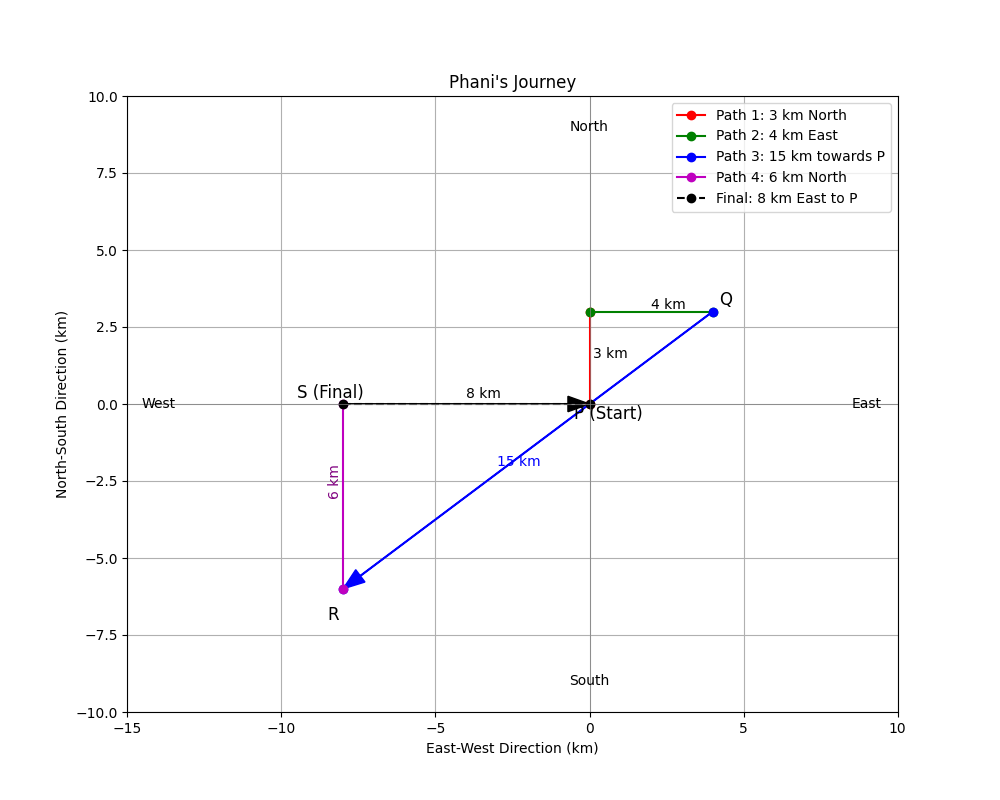
\includegraphics[width=0.85\columnwidth]{figs/graph19.png}
    \caption{12.26}
    \label{fig:placeholder}
\end{figure}
\end{document}
